\documentclass[12pt, twoside]{report}
\usepackage[utf8]{inputenc}
\usepackage[margin=2.5cm]{geometry}
\usepackage{graphicx}  		% display images
\usepackage{rotating}
\usepackage{tikz} 
\usepackage[portuguese]{babel}

\usepackage{mathptmx}
\usepackage{setspace}

\usepackage[colorlinks=true,linkcolor=black,urlcolor=blue,bookmarksopen=true]{hyperref} % Make hyperlinks in index
\usepackage{bookmark} 		% Bookmarks for pdf file
\usepackage{float} 			% colocar as imegens e tabelas dentro do texto
\usepackage{fancyhdr}
\pagestyle{fancy}
\usepackage{tabularx} 		% x column in table can jump a line
\usepackage{setspace} 		% espçamento entre linhas
\usepackage{fancyhdr} 		% creates fancy footers and headers
\raggedbottom				% makes bottom of page more empy to make sure previous text doesnt have vertical gaps
\usepackage{ltablex}
\usepackage{pdflscape}
\usepackage{multirow}
\usepackage{minted} %colocação de códigos
\pagestyle{fancy}
\lfoot{{\footnotesize Tecnologias de Informação}}
\rfoot{{\footnotesize ESTGA}}
\rhead{PTDW}
\lfoot{Calendário de exames}
\usepackage{nomencl}
\makenomenclature
\renewcommand{\nomname}{Nomenclatura}%mudar o nome da secção

\renewcommand{\footrulewidth}{1pt}%criar uma linha no que separa o rodapé

\renewcommand\listoflistingscaption{Índices dos comandos e configurações} %lista dos codigos



\begin{document}
	
\onehalfspacing % espaçamento de 1,5 entre linhas

	\pagenumbering{roman}
	
	\begin{titlepage}
		\centering
		\scshape\Huge Calendário Exames\par
		\vspace{0.9cm}
		
		\scshape\large Projeto em Tecnologias da Informação \\
		\vspace{0.3cm}
		\scshape\large 1º semestre de 2021/2022\par
		\vspace{0.4cm}
		\centering
		
		\vspace{3cm}
		
		\large
		Autor\\
		Sofia Rocha, Nº 99991 \\
		
		\vspace{2cm}
		\large
		Águeda, mês, 2022 \\
		
		\vspace{4cm}
		
		\centering
		
\includegraphics[width=10cm]{image/AssB_vertical_cor.png}
		
		
		\newpage
		\thispagestyle{plain}%retira cabeçalho e rodape
		\thispagestyle{empty}%retira a numeração da pagina
		\centering
		\scshape\Huge Calendário Exames \par
		\vspace{1cm}
		
		\scshape\large Projeto em Tecnologias da Informação\par
		\vspace{1cm}
		\scshape\large 2º semestre de 2021/2022\par
		\vspace{4cm}
		
		\large
		Autor\\
		Sofia Rocha, Nº 99991 \\
		
		\vspace{1cm}
		Orientador\\
		Fábio Marques\\
		
		\vspace{3cm}
		\large
		Águeda, mês, 2022 \\
		
		\vspace{2cm}
		\centering
		
\includegraphics[width=10cm]{image/AssB_vertical_cor}
		
	\end{titlepage}

	\begin{abstract}
	\setstretch{1.5}
	\setlength{\parskip}{14pt}
	\setlength{\parindent}{0pt}
	
	
	Resumo máximo 300 palavras
	palavras-chave (6 no máximo)
	\end{abstract}
	
	\begin{abstract}
		Resumo em inglês máximo 300 palavras
		palavras-chave (6 no máximo)
	\end{abstract}

	\newpage
	\setcounter{page}{1} % começa a contar a paginas no numero 1
	\tableofcontents % Índice de conteúdos
	\thispagestyle{plain} % retira cabeçalho e rodape
	\thispagestyle{empty} % retira a numeração da pagina
	\newpage
	\listoftables % Lista de tabelas
	\newpage
	\listoffigures % Lista de figuras
	
	
	\newpage
	\pagenumbering{arabic}
	

	\chapter{Introdução}
	\setstretch{1.5}
	\setlength{\parskip}{14pt}
	\setlength{\parindent}{0pt}
	
	Como escolha do tema para este projeto final foi apresentado a proposta de continuação do projeto no âmbito do Projeto Temático em Desenvolvimento Web associado às disciplinas Web Design e
	Desenvolvimento Web Multiplataforma em que consistia na a criação de uma aplicação web para proporcionar uma alternativa às ferramentas utilizadas atualmente por um cliente. O grupo constituinte deste projeto acordou abordar o tema de gestão de calendários de avaliações que consiste no desenvolvimento de uma aplicação web desenvolvida com as tecnologias web lecionadas no módulo temático
	que engloba este projecto. 
	
	Este relatório está dividido em quatro etapas: a revisão do projeto - verificação de \textit{bugs} e o que falta implementar, a criação de requisitos funcionais e não funcionais, correção dos \textit{bugs} encontrados e implementação de novas funcionalidades.

	
	\chapter{Planificação do projeto}
	\section{Revisão do estado do projeto}
	
		Antes de começar a implementar novas funcionalidades foi feita uma revisão de todo o projeto, a partir dos requisitos identificados no semestre passado (ver tabela \ref{requisitiosfuncionaisrevisao}), para identificar que funcionalidades necessitavam de revisões e correções de erros e quais não foram implementadas do planeamento inicial.
		
		
	\def\arraystretch{1.5}
	\begin{center}
		\label{requisitiosfuncionaisrevisao}
		\begin{longtable}{|m{1cm}|m{2.2cm}|m{9cm}|m{3cm}|}
			\caption{Requisitos funcionais implementados e não implementados}\\
			
			\hline			
			\textbf{Refª }	& \textbf{Categoria}&\textbf{Descrição do requisito} & \textbf{Implementado?} \\
			\hline
			
			RF.1 &Importação& Importação de ficheiros com a configuração de salas, disciplinas e docentes em formato \textbf{csv} & Sim \\
			\hline
			
			RF.2 &\multirow{2}{2cm}{Exportação}& Exportação de calendários em formato \textbf{pdf} & Não \\
			
			RF.3 && Exportação o calendário em língua inglesa & Não \\
			\hline
			
			RF.4 &\multirow{3}{2cm}{Marcação de exames}& Os exames podem ser marcados em três turnos: às 9h30, às 14h e às 18h30 & Sim \\
			
			RF.5 && Associação de um ou mais vigilantes a cada exame & Não \\
			
			RF.6 && O calendário não deverá permitir a marcação de exames aos domingos e feriados & Não \\
			
			RF.7 &&	Associação de uma ou mais salas a cada exame & Não\\
			
			RF.8 && Se houver vários cursos com o mesmo exame então será associado a todos os calendários dos cursos associados. & Não\\
			\hline
			
			RF.9 &\multirow{7}{2cm}{Configurações}& Configuração do tipo de sala (informática, laboratório de redes e normal) e lotação máxima & Não \\
			
			RF.10 & & Inserção de cursos e disciplinas & Não\\
			
			RF.11 && Permitir inserir novos docentes & Não\\
			
			RF.12 && Permitir editar informações (nome, que disciplinas está a lecionar, horário de trabalho) sobre os docentes & Não\\
			
			RF.13 && Permitir editar informações (nome do curso, docente e a disciplina) sobre as disciplinas e cursos & Não\\
			
			RF.14 && Alterar a disponibilidade dos docentes & Não\\
			
			RF.15 && Permitir colocar restrições arbitrárias introduzidas pelo utilizador & Não \\
			\hline	
			
			RF.16 &\multirow{9}{2cm}{Avisos}& Aparecimento de um aviso no caso de incongruência da informação durante a marcação de exames & Não \\
			
			RF.17 &&Mostrar um aviso de alta prioridade se houver sobreposições de exames & Não\\
			
			RF.18 && Mostrar um aviso de alta prioridade se o docente não estiver disponível & Não \\
			
			RF.19 && Mostrar um aviso de alta prioridade se a sala não estiver disponível & Não\\
			
			RF.20 && Mostrar um aviso de alta prioridade se o curso for diurno e colocar um exame no turno da noite e vice-versa & Não\\
			
			RF.21&&Mostrar um aviso de alta prioridade se o docente associado ao mesmo exame for repetido & Não \\
			
			RF.22 && Mostrar um aviso de alta prioridade se o exame necessitar de uma sala de informática e não for associada sala desse tipo & Não\\
			
			RF.23 && Mostrar um aviso de alta prioridade se houver mais alunos inscritos do que  lotação máxima da sala & Não\\
			
			RF.24 && Mostrar um aviso de média prioridade se houver exames marcados no mesmo dia e hora do mesmo curso mas anos diferentes & Não\\
			
			
			RF.25 && Mostrar um aviso de média prioridade se o utilizador tentar exportar um calendário sem exames marcados & Não\\
			\hline
			
			RF.26 &Autenticação& O utilizador só pode aceder à aplicação após a autenticação & Sim\\
			\hline
			
			RF.27 &\multirow{3}{2cm}{Criação de calendários}&Criação de calendários associados a um curso, ano letivo, ano do curso, época e semestre.& Sim \\
			
			RF.28 && Criação de épocas de avaliação adicionando um nome e uma data de início e fim & Não \\
			
			RF.29 && A criação de um novo calendário deverá sempre partir do início sem exames marcados & Sim\\
			\hline
			RF.30 &\multirow{2}{*}{Histórico}& Guardar e visualizar calendários de exames de anos anteriores (histórico)& Não \\
			
			RF.31 && Filtrar o histórico por curso, ano letivo, ano do curso, semestre e época& Não \\
			\hline
		\end{longtable}
	\end{center}
	
	Apesar de haver várias funcionalidades implementadas algumas destas necessitavam de correção de \textit{bugs}, apresentado na tabela \ref{revisaodaaplicacaobugs}, que prejudicavam a segurança da aplicação ou o comprometimento da funcionalidade. Os requisitos relacionados são referentes à tabela \ref{requisitiosfuncionaisrevisao}.
	
		\begin{table}[H]
		\caption{Requisitos que têm \textit{bugs}}
		
		\begin{center}
			\begin{tabularx}{\textwidth}{|X|X|}
				\hline
				\textbf{Descrição do \textit{bug}} & \textbf{Req. relacionado} \\
				\hline
				O utilizador consegue aceder à aplicação sem autenticação através do url & RF.26\\
				\hline
				Aparece várias vezes o mesmo ano do curso & RF.27\\
				\hline
				Não importa se tiver mais de um professor & RF.1\\
				\hline
				Não verifica se tem dados na base de dados & RF.1\\
				\hline
			\end{tabularx}
			\label{revisaodaaplicacaobugs}
		\end{center}
	\end{table}
	
	\section{Planeamento do projeto}
	
	A partir da revisão feita anteriormente foi possível planear todo o projeto como se pode verificar na figura 
	\ref{planeamentoinicial}.
	
		\clearpage
	\begin{landscape}
		\pagestyle{empty}
		
		\begin{figure}[H] 
			\centering 			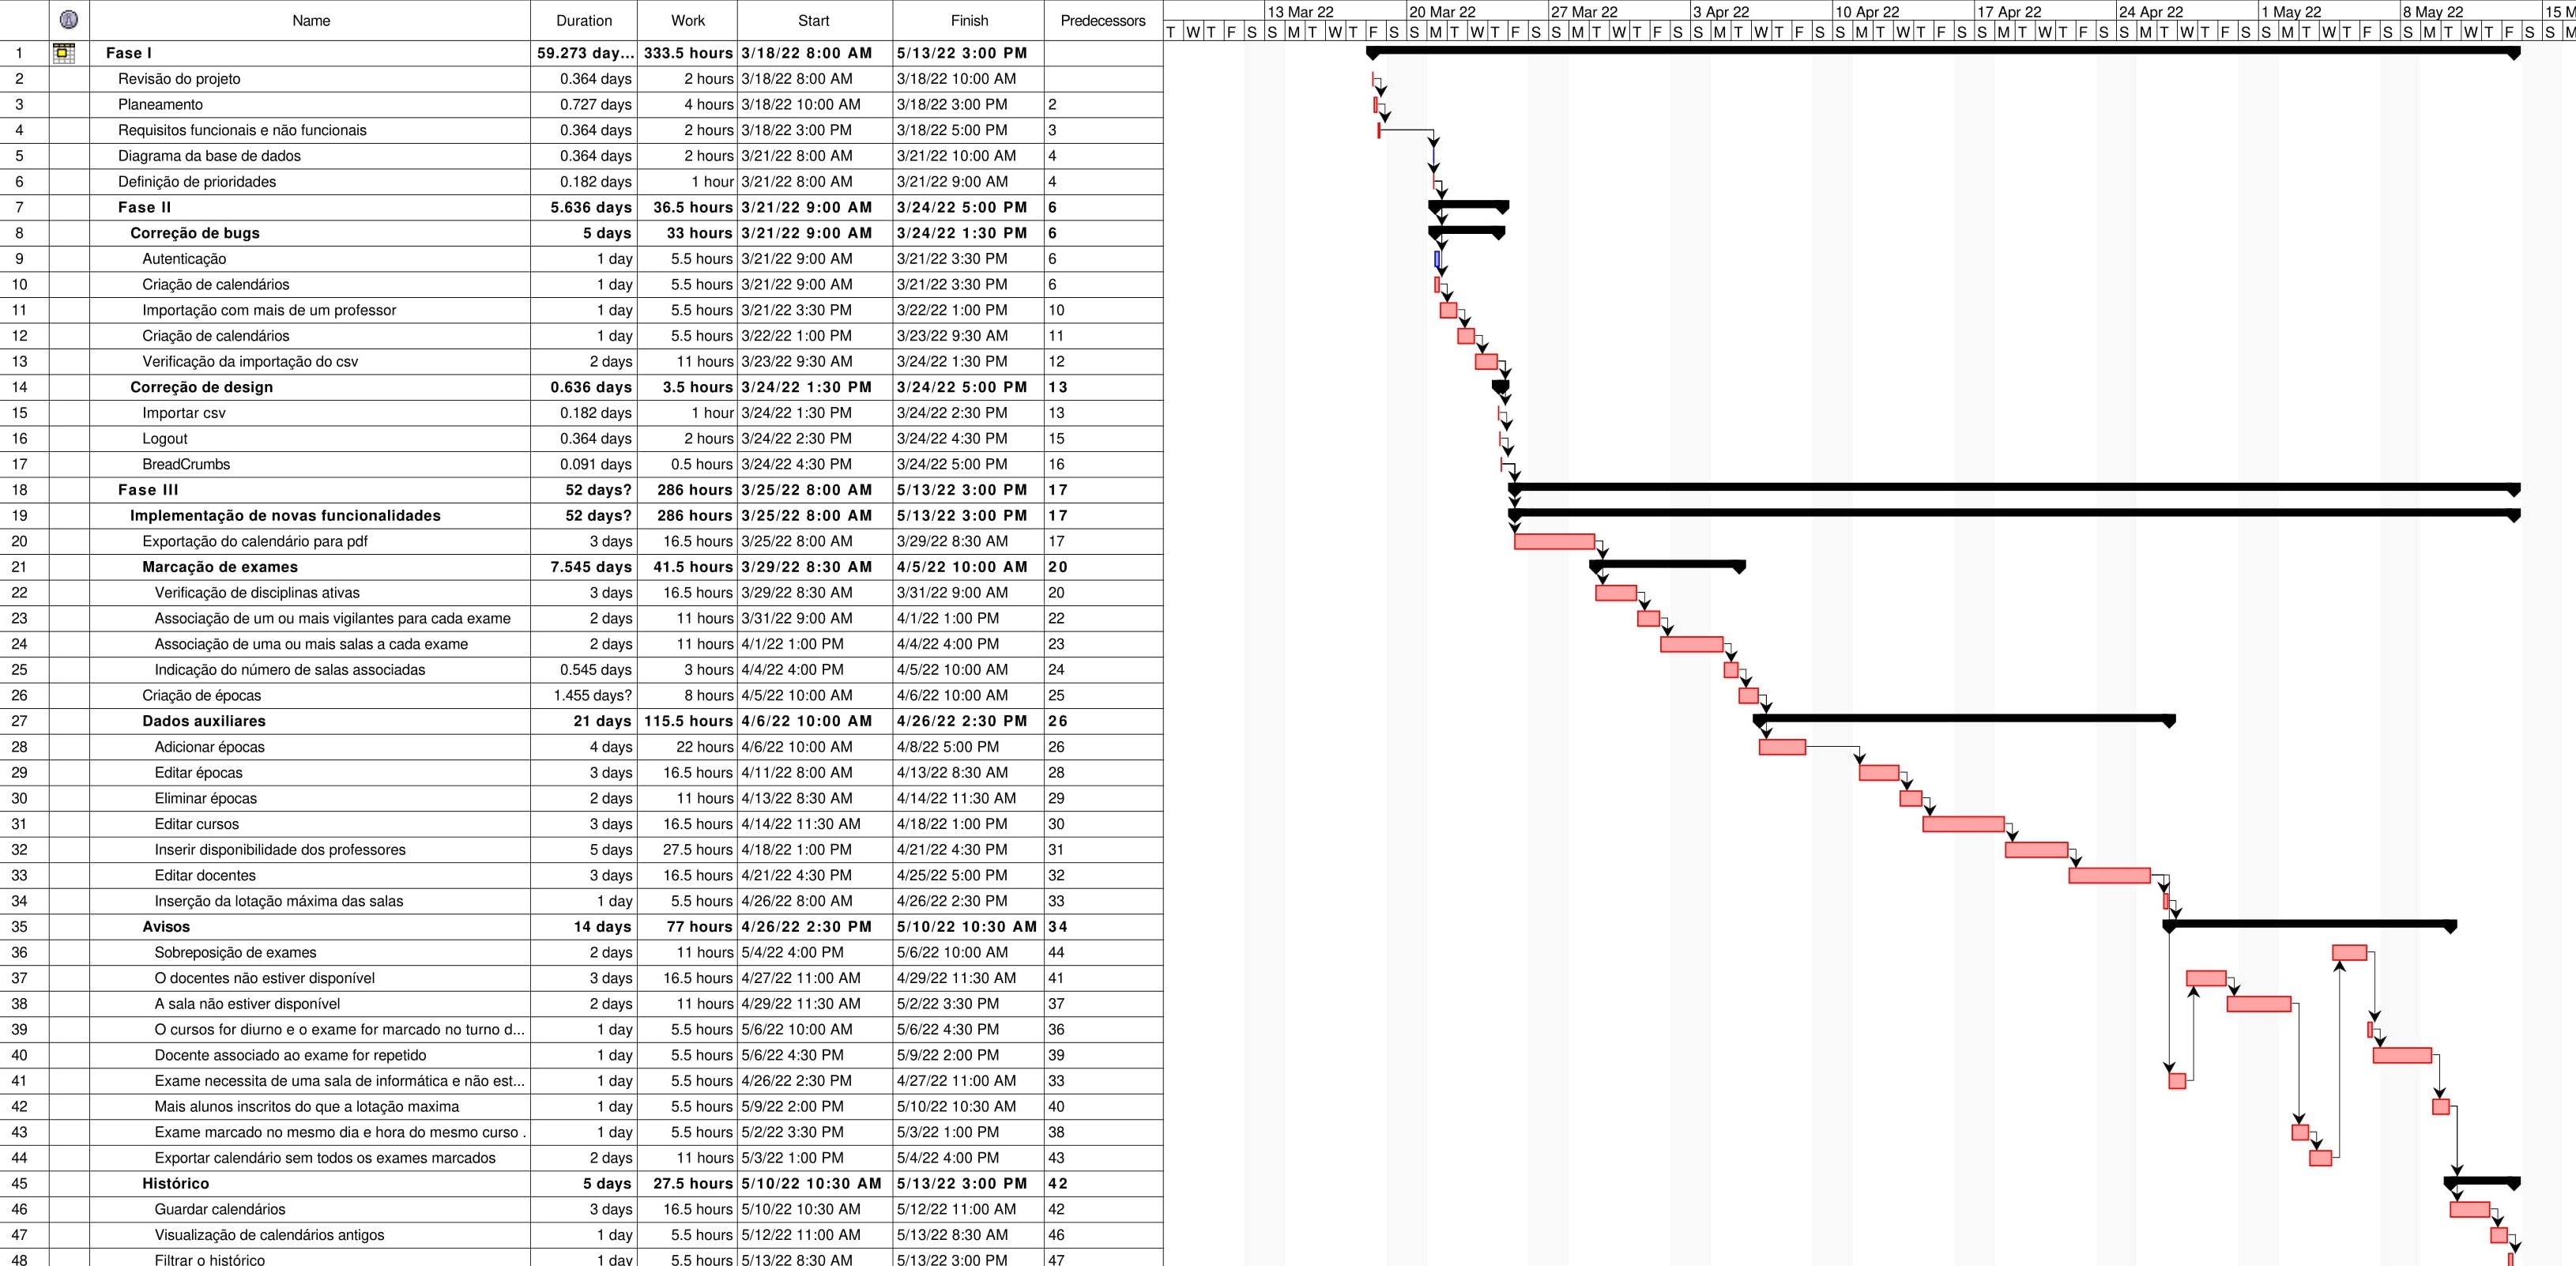
\includegraphics[width=1.4\textwidth,height=1.4\textheight,keepaspectratio]{image/planeamentoInicial}
			\caption{Planeamento do projeto}
			\label{planeamentoinicial}
			
		\end{figure}
		
		
	\end{landscape}
	\chapter{Modelo de requisitos}
	\label{requisitos}
	\section{Requisitos funcionais}
	
	Como este projeto é uma continuação de um projeto anterior então na tabela \ref{requisitiosfuncionais} não se encontram todos os requisitos funcionais, mas sim aqueles que serão implementados. 
	
	
\def\arraystretch{1.5}
	\begin{center}
		\label{requisitiosfuncionais}
		\begin{longtable}{|m{1cm}|m{2.2cm}|m{10cm}|m{2cm}|}
			\caption{Requisitos funcionais a serem implementados}\\
			
			\hline			
			\textbf{Refª }	& \textbf{Categoria}&\textbf{Descrição do requisito} & \textbf{Prioridade} \\
			\hline
			
			
			RF.1 &Importação& Importação de ficheiros com a configuração de salas, disciplinas e docentes em formato \textbf{csv} com dois ou mais docentes& Alta \\
			\hline
			
			RF.2 &\multirow{2}{2cm}{Exportação}& Exportação de calendários em formato \textbf{pdf} & Alta \\
			
			RF.3 && Exportação o calendário em língua inglesa & Baixa \\
			\hline
			
			RF.4 &\multirow{2}{2cm}{Marcação de exames}& Associação de um ou mais vigilantes a cada exame & Alta\\
						
			RF.5 &&	Associação de uma ou mais salas a cada exame & Alta\\
			
			RF.6 &&Indicação do número de salas associadas & Alta\\
			\hline
		
			RF.9 &\multirow{6}{2cm}{Dados Auxiliares}& Inserção da lotação máxima das salas& Média \\
			
			RF.10 && Alterar a disponibilidade dos docentes & Alta\\
			
			RF.10 && Adicionar épocas & Alta\\
			
			RF.11 && Editar épocas & Média\\
			
			RF.12 && Eliminar épocas & Alta\\
			
			RF.13 && Inserir disponibilidade dos docentes & Alta\\
			\hline
			
			RF.16 &\multirow{9}{2cm}{Avisos}& Mostrar um aviso de alta prioridade se houver sobreposições de exames & Baixa\\
						
			RF.17 && Mostrar um aviso de alta prioridade se o docente não estiver disponível & Média \\
			
			RF.18 && Mostrar um aviso de alta prioridade se a sala não estiver disponível & Média\\
			
			RF.19 && Mostrar um aviso de alta prioridade se o curso for diurno e colocar um exame no turno da noite e vice-versa & Baixa\\
			
			RF.20&&Mostrar um aviso de alta prioridade se o docente associado ao mesmo exame for repetido & Alta \\
			
			RF.21 && Mostrar um aviso de alta prioridade se o exame necessitar de uma sala de informática e não for associada sala desse tipo & Alta\\
			
			RF.22 && Mostrar um aviso de alta prioridade se houver mais alunos inscritos do que  lotação máxima da sala & Baixa\\
			
			RF.23 && Mostrar um aviso de média prioridade se houver exames marcados no mesmo dia e hora do mesmo curso mas anos diferentes & Média\\
			
			RF.24 && Mostrar um aviso de média prioridade se o utilizador tentar exportar um calendário sem todos os exames marcados & Média\\
			
			\hline
			
			RF.25 &Autenticação& O utilizador só pode aceder à aplicação após a autenticação & Alta\\
			\hline
			
			RF.26 &\multirow{1}{2cm}{Criação de calendários}& Criação de épocas de avaliação adicionando um nome e uma data de início e fim & Alta \\
	
			\hline
			RF.30 &\multirow{2}{*}{Histórico}& Guardar e visualizar calendários de exames de anos anteriores (histórico)& Média \\
			
			RF.31 && Filtrar o histórico por curso, ano letivo, ano do curso, semestre e época& Média \\
			\hline
		\end{longtable}
	\end{center}



	
	\section{Requisitos não funcionais}
	
	Os requisitos não funcionais estão divididos em três categorias: requisitos de interface e facilidade de uso que representam todos os requisitos que melhorem a usabilidade da aplicação; requisitos de segurança e integridade dos dados e requisitos de interface com sistemas externos e ambientes de execução.
	
	\subsection{Requisitos de interface e facilidade de uso}

Assim que o utilizador inicia a sessão na aplicação este tem de facilmente entender como a aplicação está organizada.
Isto permite que o utilizador utilize a aplicação durante mais tempo e gerir os calendários de avaliações não seja frustrante.
	
	\begin{table}[H]
	\caption{Requisitos de interface e facilidade de uso}
	
	\begin{center}
		\begin{tabularx}{\textwidth}{|c|X|c|}
			\hline
			\textbf{Refª }	& \textbf{Descrição do requisito} & \textbf{Prioridade} \\
			\hline
			RIF1 & As disciplinas e cursos podem ser inseridas através de \textit{drag e drop} &Alta\\
			\hline
			RIF2 & Interface responsivo permitindo a sua visualização em ambiente mobile &Alta\\
			\hline
			RIF3 & Linguagem padrão em Português de Portugal &Alta\\
			\hline
			RIF4 & Há dois tipos de avisos distinguidos com texto e cor &Alta\\
			\hline
		\end{tabularx}
		\label{requisitosdeinterface}
	\end{center}
	\end{table}

	\subsection{Requisitos de segurança e integridade dos dados}
	
	Para que o utilizador possa colocar os seus dados na aplicação sem conter risco de vazar para utilizadores indesejados foram criados alguns requisitos de segurança referido na	tabela \ref{requisitosdeseguranca}.
	
\begin{table}[H]	
	\caption{Requisitos de segurança e integridade dos dados}
	
	
	\begin{center}
		\begin{tabularx}{\textwidth}{|c|X|c|}
			\hline
			\textbf{Refª }	& \textbf{Descrição do requisito} & \textbf{Prioridade} \\
			\hline
			RSI1 &O histórico não pode ter associações a outras tabelas da base de dados  &Alta\\
			\hline
			RSI2 & Uma única conta de utilizador&Alta\\
			\hline
		\end{tabularx}
		\label{requisitosdeseguranca}
	\end{center}
\end{table}


	\subsection{Requisitos de interface com sistemas externos e ambientes de execução}
	
	A aplicação por ambiente da disciplina irá ser programada em linguagens web,
	consequentemente não é necessário definir que sistema operativos pode a aplicação ser executada.
	No entanto é crucial ter acesso à rede da Universidade de Aveiro e um dos navegadores definidos na tabela \ref{requisitosdesistemas}.
	
	\def\arraystretch{1.5}
	\begin{table}[H]
		\caption{Requisitos de interface com sistemas externos e ambientes de execução}
		\begin{center}
			\begin{tabularx}{\textwidth}{|c|X|c|}
				\hline
				\textbf{Refª }	& \textbf{Descrição do requisito} & \textbf{Prioridade}\\
				\hline
				RSA1 & Suportar Browsers com motor renderização webkit/blink (Chrome, Edge, Safari, Brave, etc.)  & Alta \\
				\hline
				RSA2 & Suportar Firefox ESR e outros derivados de gecko/quantum & Alta \\
				\hline
				RSA5 & Estar conectado à rede da Universidade de Aveiro & Alta\\
				\hline
			\end{tabularx}
			\label{requisitosdesistemas}
		\end{center}
	\end{table}
		
	

	
	
	\chapter{Modelo de dados persistentes}
	
		Para cumprir com as novas funcionalidades, apresentados anteriormente na secção \ref{requisitos}, a base de dados teve de ser alterada. 
	
	\section{Estrutura da base de dados}
	
	Para a preparação da aplicação a tabela ``course" é preenchida com todos os cursos da universidade a partir da própria \textit{framework} assim como ``time\_slot" que contém somente os três blocos em que se pode marcar um exame (manhã, tarde e noite).
	
	De seguida, Para utilizar a aplicação o utilizador terá de se autenticar com a sua conta (se não tiver terá de se registar) que está registada na tabela ``users". No entanto não existe nenhuma associação dos dados às contas sendo que todas as contas têm acesso ao mesmos dados.
	
	Depois o utilizador terá de importar o csv em que os dados serão guardados nas tabelas ``professor", ``subject" e ``classroom". Se existir mais que um professor para uma disciplina, estes serão guardados na tabela ``professor", mas só será associado à disciplina o primeiro que aparece no ficheiro .csv uma vez que se assume que é o representante da mesma.
	
	Com isto todos os calendários criados serão armazenados na tabela ``calendar" que contém duas chaves estrangeiras para a época e para o curso para os quais foram associados. As épocas (criadas pelo utilizador) são identificadas pelo seu nome, data de início e fim. Para cada calendário existe inúmeros exames que podem ser marcados (tabela ``evaluation\_slot´´) consoante o curso associado. Cada exame tem três chaves estrangeiras: uma para o calendário, outra para a disciplina e outra para o momento do dia em que será a avaliação e um atributo para o dia marcado.
	
	Nesta fase foi alterada a base de dados criando duas tabelas - ``observing\_professor", que guarda todos os vigilantes associados a um exame, e ``associated\_classroom", que armazena todos as salas de um exame - para que possa ser associado um ou mais vigilantes ou uma ou mais salas a cada exame (RF.2 e RF.3 da tabela \ref{requisitiosfuncionais}).
	
	\clearpage
	\begin{landscape}
		\pagestyle{empty}
		
		\begin{figure}[H] 
			\centering 			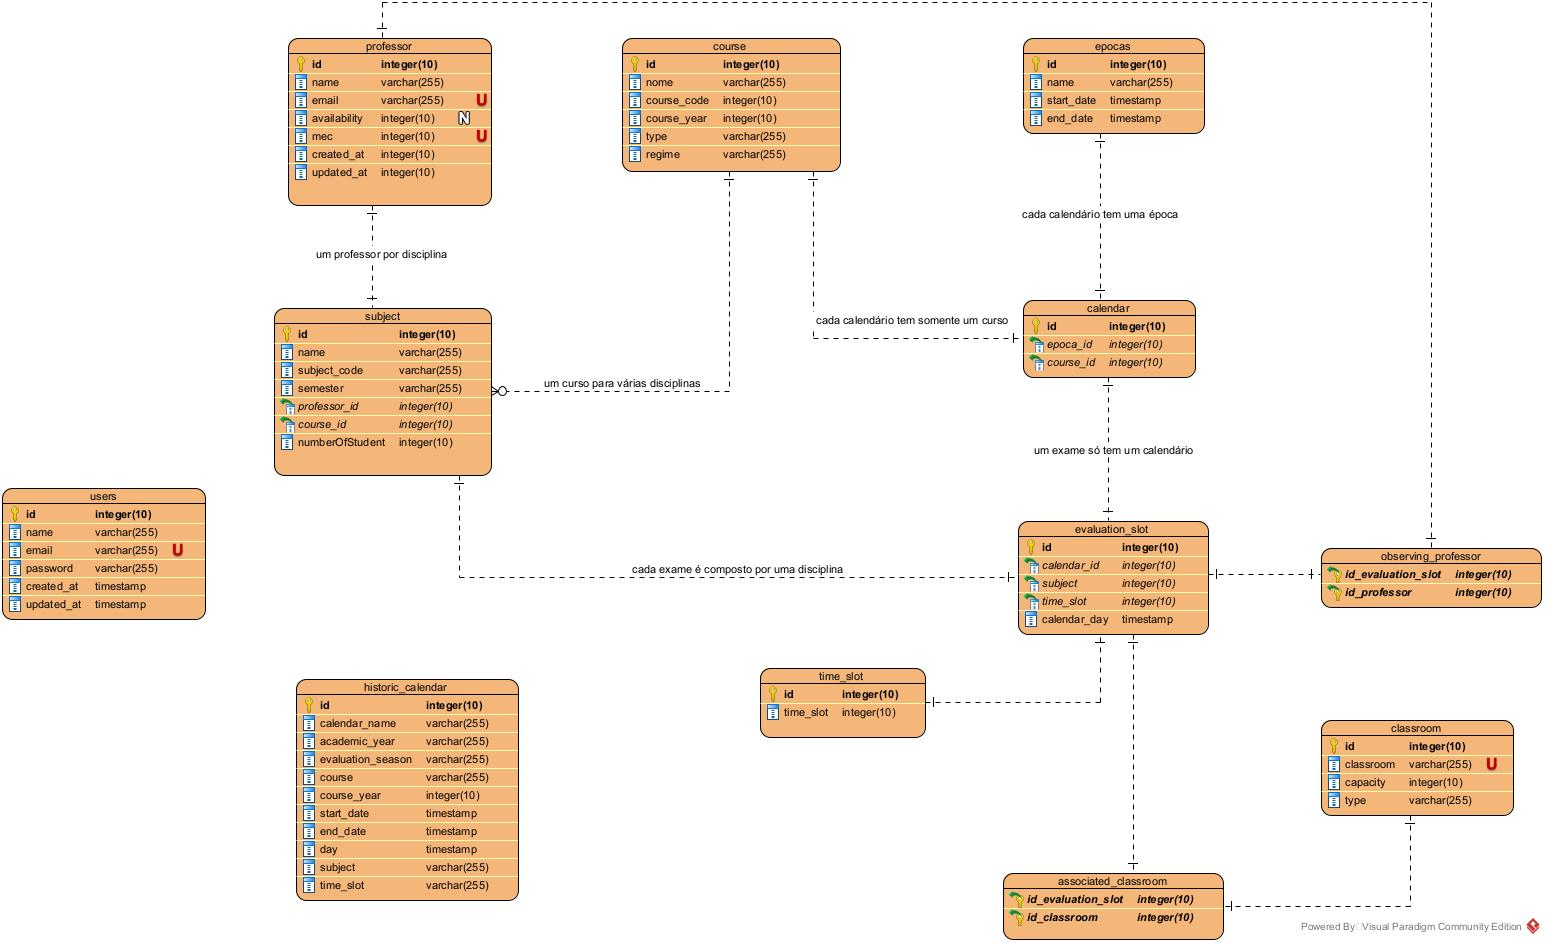
\includegraphics[width=1.4\textwidth,height=1.4\textheight,keepaspectratio]{image/databaseDiagram}
			\caption{Diagrama da base de dados}
			\label{planeamentoinicial}
			
		\end{figure}
		
		
	\end{landscape}
	
	\section{Arquitetura do sistema - modelo MCV}
	
	
	\section{Correção de erros}

	\subsection{Autenticação}
	No começo foi bloqueado o acesso à aplicação através do próprio do url do website. Por exemplo era possível aceder à página de marcação de exames digitando "/marcacao-exames" sem iniciar sessão. 
	Consequentemente, de forma a corrigir este problema, antes de aceder a qualquer rota (exceto a de login e de registo) é verificado se existe uma sessão aberta através do \textit{middleware}, como se pode verificar no código \ref{routesMiddl} e \ref{autenticarMiddl}.
	
	\begin{listing}[H]
	\begin{minted}[
		frame=lines,
		framesep=2mm,
		baselinestretch=1,
		fontsize=\footnotesize,
		linenos
		]{php}
	Route::middleware([Authenticate::class])->group(function (){
	
	\end{minted}
	\caption{Verificação através do \textit{middleware} se o utilizador está autenticado}
	\label{routesMiddl}
	\end{listing}                                 
		
	\begin{listing}[H]
	\begin{minted}[
		frame=lines,
		framesep=2mm,
		baselinestretch=1,
		fontsize=\footnotesize,
		linenos
		]{php}
	class Authenticate extends Middleware
	{
	/**
	* Caso o utilizador não esteje logado não permite navegar pelas páginas
	* return route
	*/
	protected function redirectTo($request)
	{
	  if (!Auth::check()) {
		return route('login');
	  }
	}
	}
				\end{minted}
				\caption{\textit{Middleware} que redireciona para a página delogin se não tiver autenticado}
				\label{autenticarMiddl}
			\end{listing}    
		
	\subsection{Importação}
	
	Na versão anterior do projeto não se considerava as disciplnas que contivessem mais de um professor, assumindo-se que o ficheiro .csv a importar nunca tivesse esta restrição. No entanto o ficheiro dado contém disciplinas com um professor representante e dois auxiliares. 
	
	Com isso o código foi alterado para verificar se existe mais de um número mecanográfico por disciplina. Se existir o primeiro será assumido como representando da disciplina sendo o único que será associado à mesma e os outros serão somentes guardados na base de dados, como está ilustrado no código \ref{importarprof}. 
	

	\begin{listing}[H]
	\begin{minted}[
		frame=lines,
		framesep=2mm,
		baselinestretch=1,
		fontsize=\footnotesize,
		linenos
		]{php}
	$mec = explode(",", $data[$i][9]);
			
	if (count($mec) > 1) {
		$name = explode(",", $data[$i][7]);
		$email = explode(",", $data[$i][8]);
				
		for ($x = 0; $x < count($mec); $x++) {
			//cria um professor ou atualiza o prof 
			se tiver o mesmo número mecanografico
			Professor::updateOrCreate([
			'mec' => $mec[$x],
			'name' => $name[$x],
			'email' => $email[$x],
			]);
		}
	}
	\end{minted}
	\caption{Importação do professores}
	\label{importarprof}
	\end{listing}
	
	\section{Verificação da importação do csv}
	
	Para o utilizador saber se já foi importado um csv este é avisado através de uma mensagem (\textit{toastr}) na página de importar o csv. 
	
	\begin{figure}[H] 
	\centering
	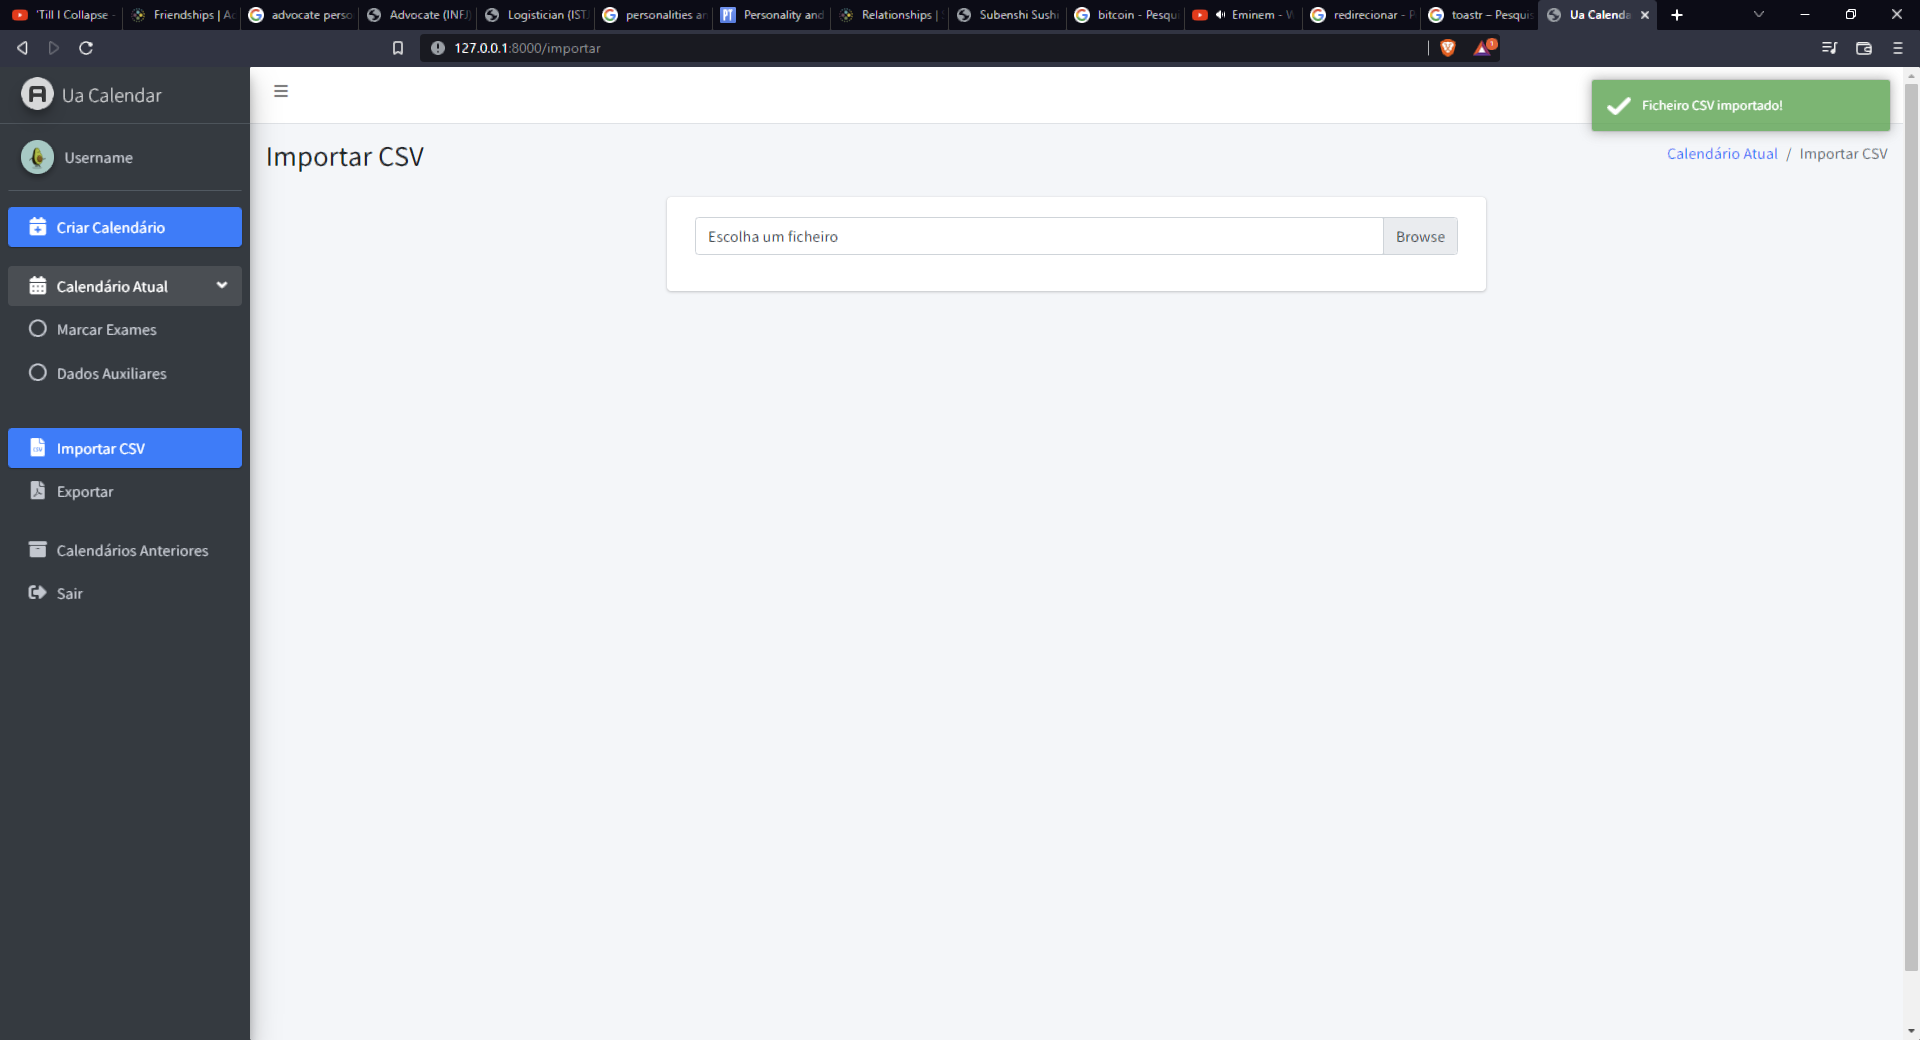
\includegraphics[width=1\textwidth,height=1\textheight,keepaspectratio]{image/importarCSV}
	\caption{\textit{Toastr} de sucesso}
	\label{importarCSVSucess}
		
	\end{figure}

	\begin{figure}[H] 


	\centering 			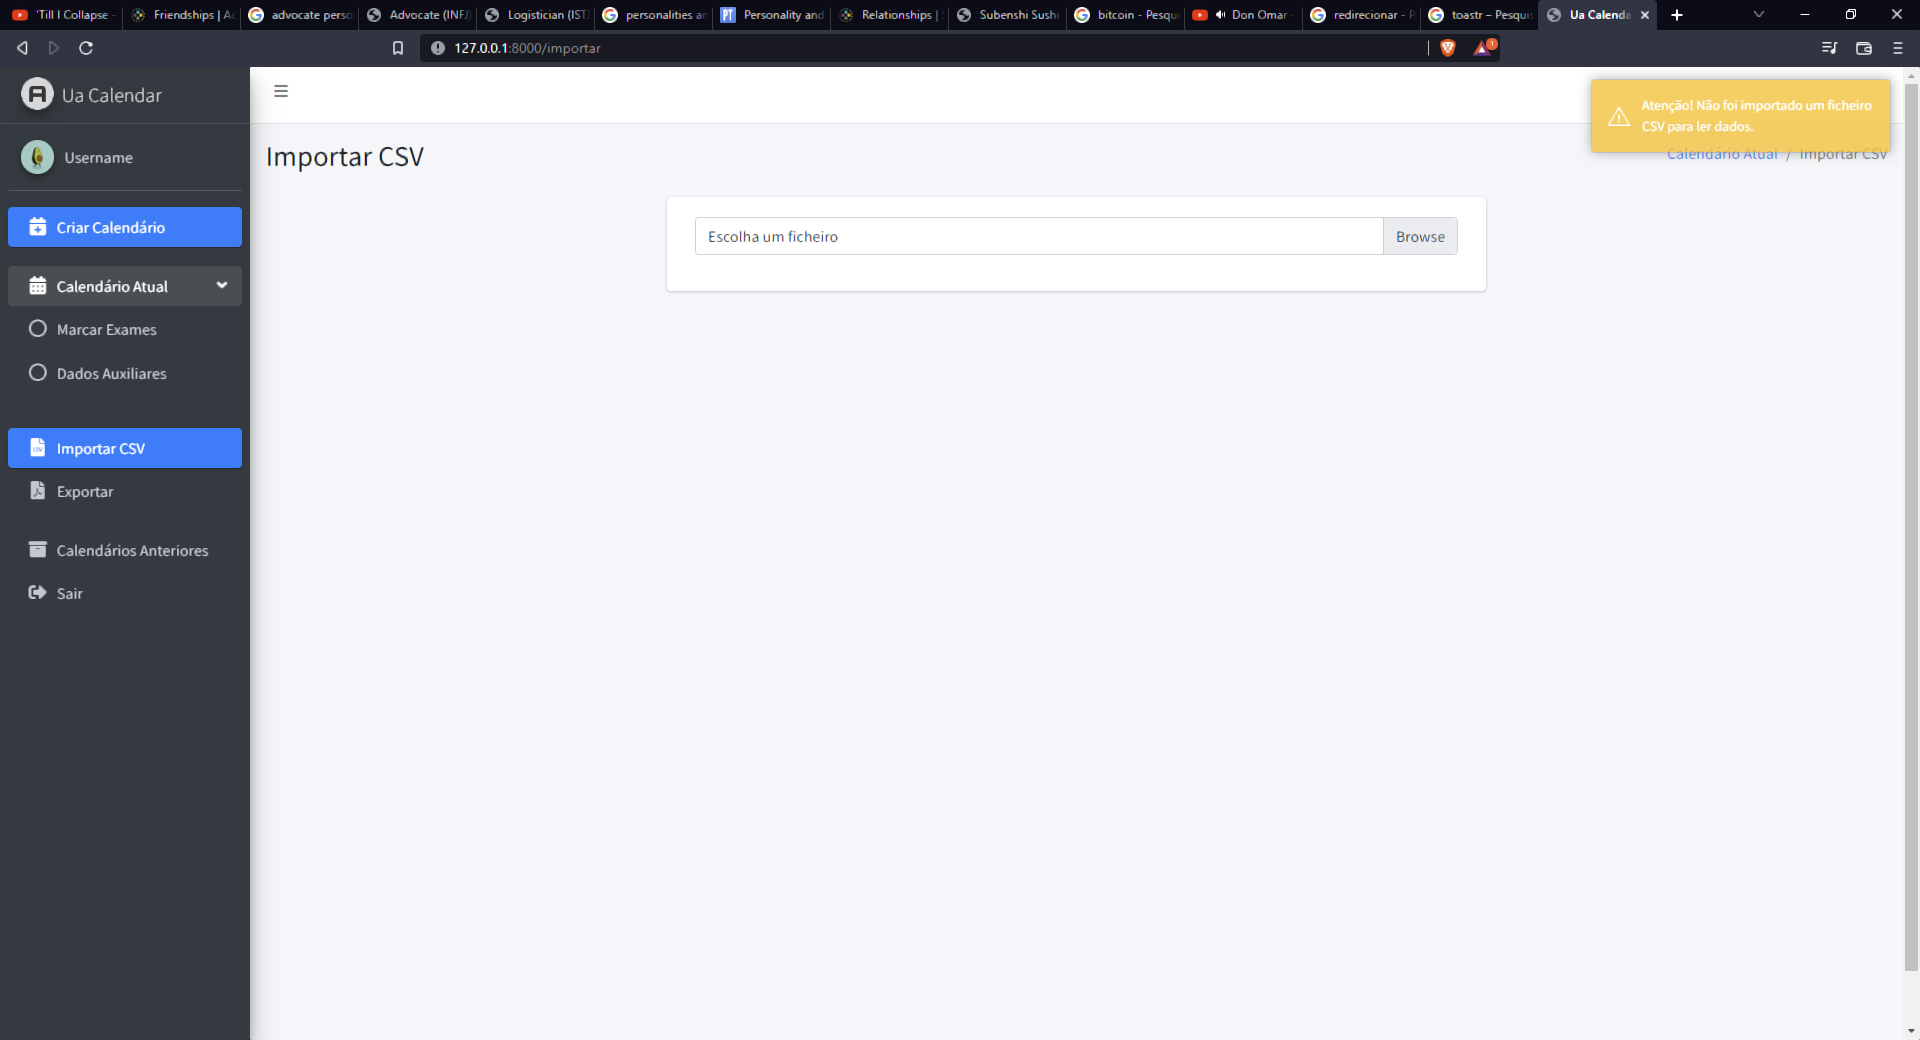
\includegraphics[width=1\textwidth,height=1\textheight,keepaspectratio]{image/importCSVFail}
	\caption{\textit{Toastr} de não ter sido importado um csv}
	\label{importarCSVFail}
	
	\end{figure}

	Este \textit{toastr} é ativado consoante os dados persentes na \textit{cookie} presente. Ao carregar a página é verificado se existe dados na base de dados através do \textit{controller} e com isso é alterado o cookie de acordo com o resultado. Como a tabela de professores é umas das que é preenchida ao importar o ficheiro .csv então se existir dados na mesma quer dizer que este ficheiro ja foi importado, através do código \ref{checkIfImported}. Apesar disto nada impede que importar mais do que uma vez.
	
	\begin{listing}[H]
		\begin{minted}[
			frame=lines,
			framesep=2mm,
			baselinestretch=1,
			fontsize=\footnotesize,
			linenos
			]{php}
		/**
		* Verifica se o csv já foi importado
		* @return bool
		*/
		public function checkIfImported()
		{
			if (Professor::exists())
			return true;
			
			return false;
		}
		\end{minted}
		\caption{Verificação se já existe dados na base de dados}
		\label{checkIfImported}
	\end{listing}
	
		
	\section{Implementação de funcionalidades}
	\subsection{Dados auxiliares}
	
	Na secção dos dados auxiliares é apresentado todos os dados da base de dados divididos em quatro categorias: Unidades curriculares, Docentes, Salas e Épocas. 
	
	\begin{figure}[H] 
		
	\centering 			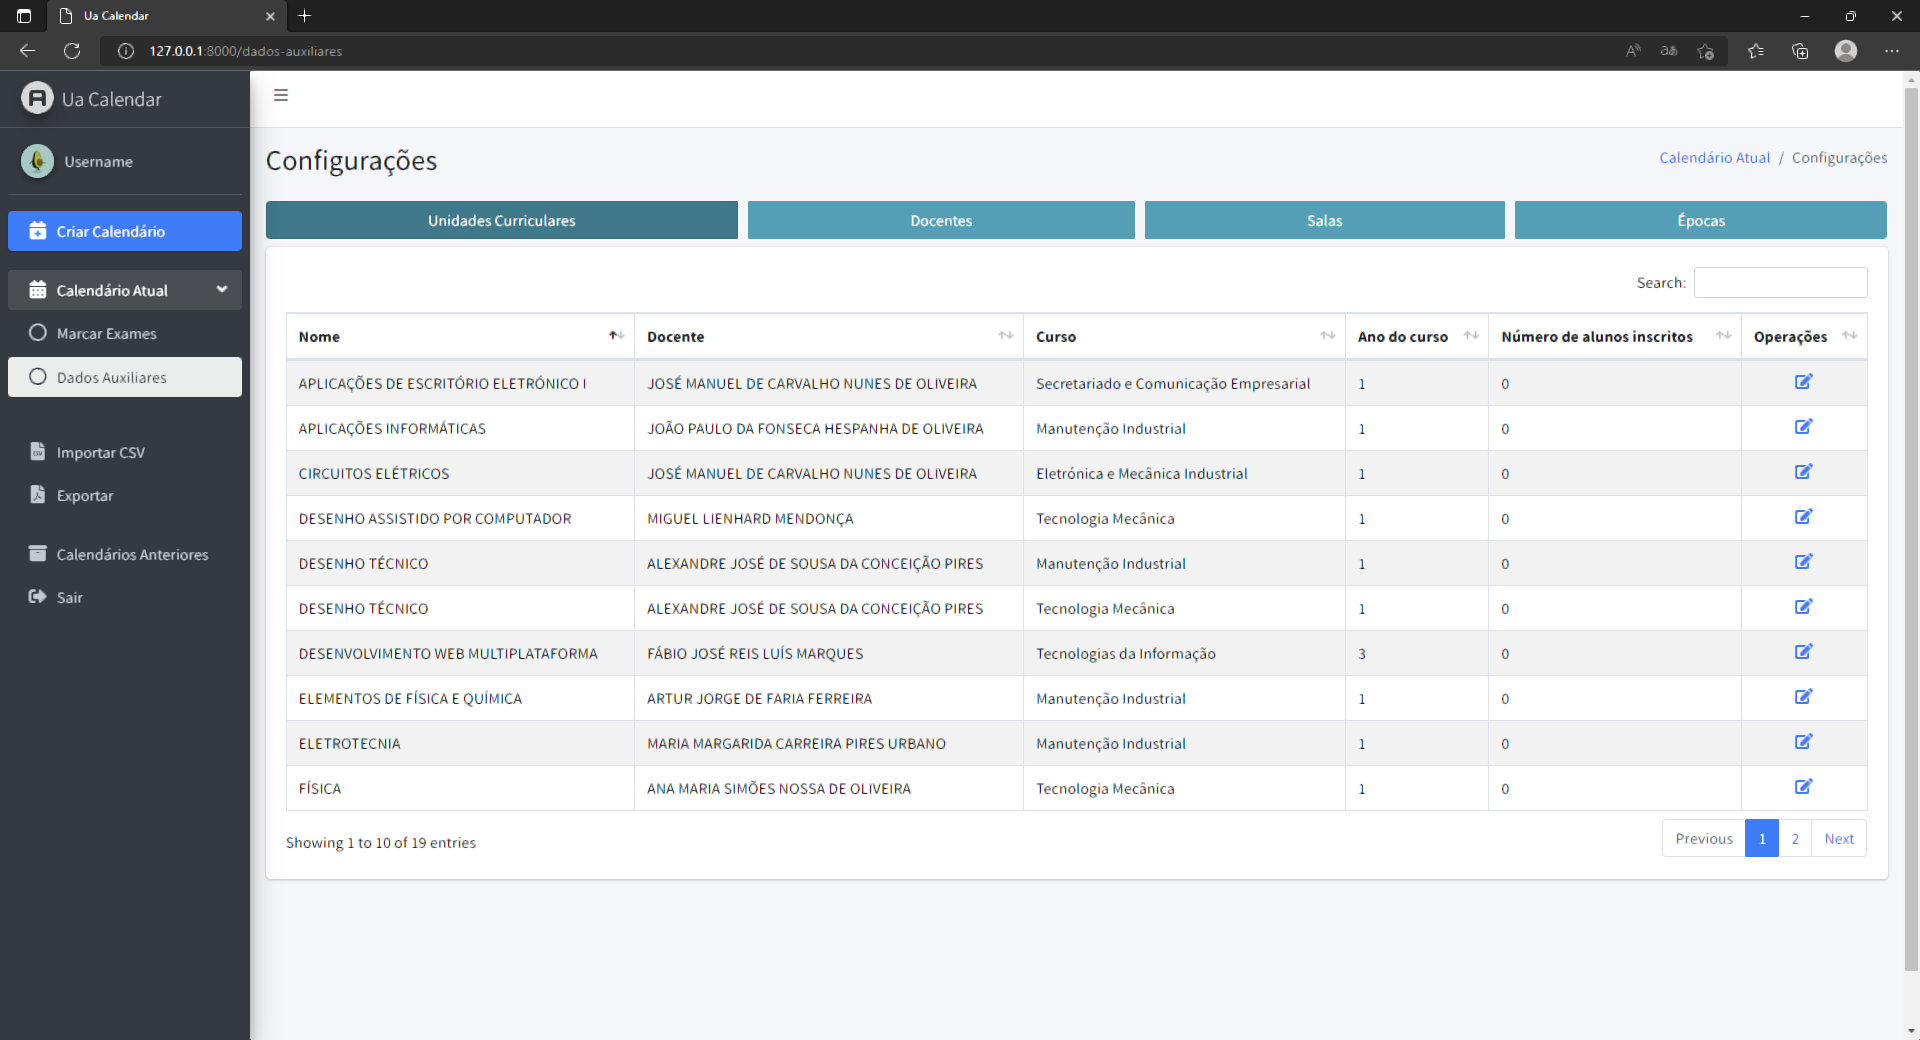
\includegraphics[width=1\textwidth,height=1\textheight,keepaspectratio]{image/dadosAuxiliares}
	\caption{Página de dados auxiliares}
	\label{dadosAuxiliares}
		
	\end{figure}
	
	Dentro dessas categorias é possível editar alguns dados. Na categoria ``Unidades Curriculares'' é possível alterar o docente da UC por outro já existente e também o número de alunos inscritos. Em ``Docentes'' qualquer dado é editável exceto disponibildade que não está implementado. Em ``Salas'' só é possível alterar a lotação da sala em exame. E por fim em ``Épocas'' é possível criar, editar ou eliminar qualquer uma.
	
	Estas operações são realizadas todas de forma semelhante. Primeiramente todos os dados apresentados são enviados a partir do controller ``ConfigurationsController'', como está apresentado em \ref{dadosController}. 
	
	\begin{listing}[H]
	\begin{minted}[
		frame=lines,
		framesep=2mm,
		baselinestretch=1,
		fontsize=\footnotesize,
		linenos
		]{php}
	public function showView()
	{
	$subjects = Subject::all();
	$professors = Professor::all();
	$classrooms = Classroom::all();
	$epocas = Epoca::all();
	$courses = Course::all();
	return view('configurations', compact(["subjects","professors",
			"classrooms","epocas","courses"
	]));
	}
	\end{minted}
	\caption{Apresentação da página de dados auxiliares a partir do controller}
	\label{dadosController}
	\end{listing}
	  
	Após isso o utilizador pode realizar qualquer uma das operações indicadas acima. Em épocas o utilizador pode criar uma nova - uma de cada vez, para evitar conflitos no controlador, como se pode ver na figura \ref{epocasAdd} - em que o procedimento começa em adicionar uma nova linha na \textit{datatable} com um campo para escrever o nome da mesma e um \textit{daterangepicker} para possa escolher o intervalo de datas para a avaliação. 
	
	\begin{figure}[H] 
		
		\centering 			
		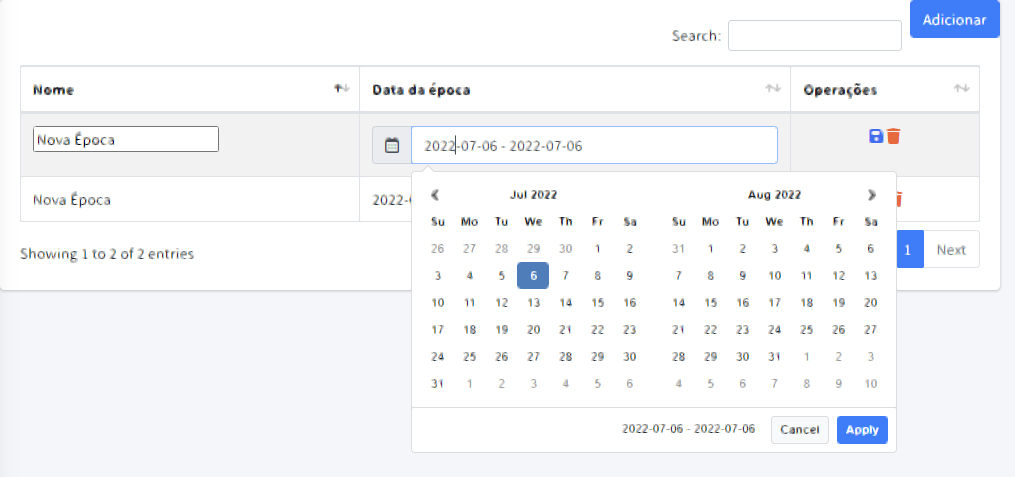
\includegraphics[width=1\textwidth,height=1\textheight,keepaspectratio]{image/epocasAdd}
		\caption{Adicionar uma época}
		\label{epocasAdd}
		
	\end{figure} 

	Para evitar cliques multiplos o \textit{event handler} é sempre removido depois deste ser acionado, como se pode ver no código \ref{epocasAddDatable}. Neste é adicionado uma nova linha com referido acima e como ete ainda não tem nenhum id na base de dados então na função ``saveEpoca'' recebe um valor nulo.
	
	\begin{listing}[H]
	\begin{minted}[
		frame=lines,
		framesep=2mm,
		baselinestretch=1,
		fontsize=\footnotesize,
		linenos
		]{javascript}
	$("#adicionarEpoca").off('click').on('click', function () {
	if (adicionarEpoca) {
	adicionarEpoca = false;
	tableEpocas.row.add([
	' <div class="data">0</div>',
	'<div class="input-group">' +
	'   <div class="input-group-prepend">' +
	'       <span class="input-group-text">' +
	'           <i class="far fa-calendar-alt"></i> ' +
	'       </span>' +
	'  </div>' +
	'  <input type="text" class="form-control float-right daterange" > </div>',
	'  <div align="center"> <a class="edit"> <i class="fas fa-edit"> </i>' +
	'  </a> <a class="save"> <i class="fas fa-save"></i> </a>' +
	'  <a class="delete"> <i class="fas fa-trash"></i> </a></div>']).draw();
	
	saveEpoca(null);
					
	\end{minted}
	\caption{Adicionar uma nova linha à tabela da secção das épocas}
	\label{epocasAddDatable}
	\end{listing}
	
	Dentro da função ``saveEpoca'' obtém-se todos os valores (nome, data de início e fim da época) da linha criada - através do seu índice - e remove todos as entradas. O índice é obtido encontrando a linha mais próxima (``tr'') do \textit{input.data} que pertence ao nome da época (linha 2, do código \ref{epocasAddControlador}). Depois através deste é substituído todos os dados para texto para deixarem de ser editáveis e enviados para o controlador, como se pode ver no código \ref{epocasAddControlador}.
 	
	\begin{listing}[H]
	\begin{minted}[
		frame=lines,
		framesep=2mm,
		baselinestretch=1,
		fontsize=\footnotesize,
		linenos
		]{javascript}
	nomeEpoca = $('#epocas').find('input.data');
	var rowIndex = tableEpocas.row($(nomeEpoca).closest('tr')).index();
		
	//o nome inserido
	var fieldName = $('#epocas').find('input.data[name="nomeEpoca"]').val();
	var fieldDate = date.val();
	dateArray = fieldDate.split("-");
			
	startDate = dateArray[0] + "-" + dateArray[1] + "-" + dateArray[2];
	endDate = dateArray[3] + "-" + dateArray[4] + "-" + dateArray[5];
	
	//remove todos os dados adicionados anteriormente
	$('#epocas').find("input.data").remove();
	$('#epocas').find("input.daterange").remove();
			
	//adiciona o novo nome a celula
	tableEpocas.cell(rowIndex, 0).data('<div id=' + idEpoca + ' class="data">' 
	+ fieldName + '</div>');
	tableEpocas.cell(rowIndex, 1).data('<div class="epoca">' + 
	startDate + " até " + endDate + '</div>');
		
	if (idEpoca == null) {
		insertNewEpoca(fieldName, startDate, endDate);
	} else {
	//update na base de dados
		updateEpoca(idEpoca, fieldName, startDate, endDate);
	}
	\end{minted}
	\caption{Obtenção e envio de todos os dados para o controlador}
	\label{epocasAddControlador}
	\end{listing}

	Como neste caso o id da época é nulo então envia-se todos os dados para o controllador e este retorna o id criado na base de dados. Este id é adiconado ao nome da época para que se possa editar a mesma no futuro, como se pode ver na resposta do ajax no código \ref{epocaAddDatabase}.
	
	\begin{listing}[H]
	\begin{minted}[
	frame=lines,
	framesep=2mm,
	baselinestretch=1,
	fontsize=\footnotesize,
	linenos
	]{javascript}
$.post("{{ route('criarEpocaConfigurations')}}",
{
	nome: JSON.stringify(fieldName),
	startDate: JSON.stringify(startDate),
	endDate: JSON.stringify(endDate),
		
}, function (response) {
	//adiciona o id da epoca
	tableEpocas.row(':first').nodes().to$().find('.data')
	.attr('id', response['idEpoca']);
})
	\end{minted}
	\caption{Envio de dados para o controlador e na resposta adicionar o id ao nome da época}
	\label{epocaAddDatabase}
	\end{listing}

	Na edição de uma época o processo é idêntico mas obtêm-se primeiramente o id da época para que todos os dados sejam alterados na base de dados na época correspondente. Da mesma forma que este mesmo id é utilizado para eliminar uma época. No entanto a tabela na base de dados está criada para ser eliminada ON CASCADE não havendo quaisquer verificações.
	
	Em suma, apesar de em todas as outras tabelas o processo ser idêntico existe uma verificação quando se edita o email e o nmec dos docentes uma vez que estes tem ser único. Caso não seja único é apresentado um aviso para o utilizador, como se pode ver no código \ref{docenteAddDatabase}.
	
	\begin{listing}[H]
	\begin{minted}[
	frame=lines,
	framesep=2mm,
	baselinestretch=1,
	fontsize=\footnotesize,
	linenos
	]{javascript}
function (response) {
//adiciona o id da epoca
if (typeof response['exception'] === "object") {
	toastr.error('Ocorreu um erro! O nmec ou o email já está a ser utilizado.');
	tableDocente.row(':first').remove().draw(false);
		
} else if (typeof response['idDocente'] === "number") {
	tableDocente.row(':first').nodes().to$().find('.nomeDocente')
	.attr('id', response['idDocente']);
}
	\end{minted}
	\caption{Verificação se o nmec e o email são únicos ao criar um docente}
	\label{docenteAddDatabase}
	\end{listing}

	\subsection{Criação de calendários}
	Na versão anterior do projeto era possível criar calendários para somente para épocas já existentes não sendo possível criar novas. Por isso adicionou-se essa funcionalidade à página ``Criar calendário'', como se pode ver na figura \ref{criarEpoca}. Este formulário está escondido e assim que o utilizador clicar em ``Adicionar época'', este aparece através da função ``showFrom()'' apresentado 
	no código \ref{addNovaEpoca}.
	
	\begin{listing}[H]
	\begin{minted}[
			frame=lines,
			framesep=2mm,
			baselinestretch=1,
			fontsize=\footnotesize,
			linenos
			]{javascript}
function showFrom() {
	let mostrarEpoca = $('#showCriarEpoca');
	let form = $('#criarEpocaForm');
			
	if (mostrarEpoca.css("display") === "none") {
		mostrarEpoca.css("display", "inline-block");
		form.css("display", "none");
	} else {
		mostrarEpoca.css("display", "none");
		form.css("display", "block");
	}
}
	\end{minted}
	\caption{Apresentação do formulário para adicionar uma nova época}
	\label{addNovaEpoca}
	\end{listing}
	
	\begin{figure}[H] 
		\centering
		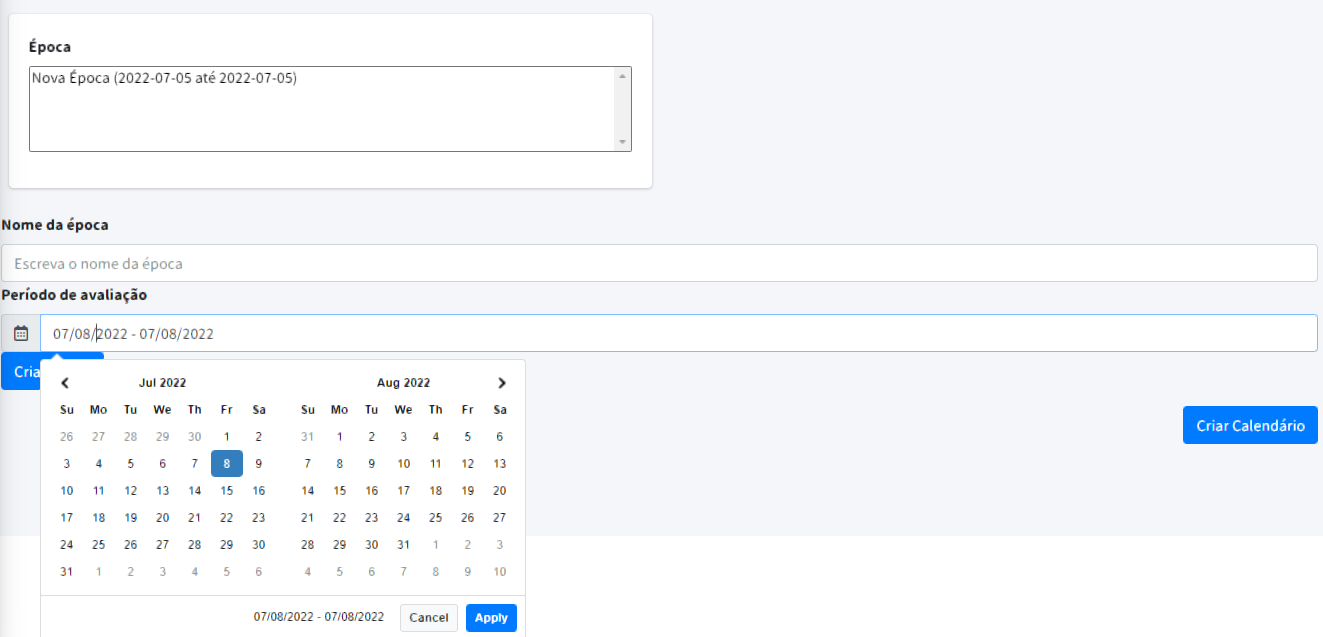
\includegraphics[width=1\textwidth,height=1\textheight,keepaspectratio]{image/criarEpoca}
		\caption{Adicionar uma nova época}
		\label{criarEpoca}
		
	\end{figure}

	\subsection{Marcação de exames}	
	
	Na página ``marcar exames'' foi alterado a forma como é obtida toda a informação sobre os exames marcados e não marcados. Na versão anterior era feito vários pedidos ao controllador à medida que era necessário causando vários conflitos. Assim, para melhorar a eficiência da aplicação, todos as informações sobre os exames (nome, dia marcado, avisos - explicado na secção \ref{avisosSeccao}, etc) são requisitadas uma única vez e recebido, do lado do cliente, em formato JSON, como se pode ver no código \ref{requestExames}.
	
	\begin{listing}[H]
		\begin{minted}[
			frame=lines,
			framesep=2mm,
			baselinestretch=1,
			fontsize=\footnotesize,
			linenos
			]{javascript}
$.post("{{ route('api-getExames')}}",
{
	codeCourse: JSON.stringify(codeCourse),
	idEpoca: JSON.stringify(idEpoca),
	yearCourse: JSON.stringify(yearCourse),
			
}, function (response) {	
	var disciplinaString = " ";
	response['exames'].forEach(element => {
		if(element['idEvaluationSlot'] == null){
			disciplinaString += "<div class='external-event bg-success'>"+
			 element['subject']['name'] + "</div>";
		}
	});
		
	$("#external-events").html(disciplinaString);
	alterarCalendario(response['exames']);
			
})
	\end{minted}
	\caption{Pedido e tratamento da resposta de todos os exames}
	\label{requestExames}
	\end{listing}

Do lado do servidor estas informações são obtidas no controlador sem a utilização dos \textit{Models} uma vez que não é possível através dos mesmos obter informações sobre tabelas que contenham uma chave primária com dois atributos. Por isso utilizou-se a biblioteca \textit{Illuminate\ Support\ Facades\ DB}, como está apresentado no código \ref{getDataDB}.

	\begin{listing}[H]
	\begin{minted}[
		frame=lines,
		framesep=2mm,
		baselinestretch=1,
		fontsize=\footnotesize,
		linenos
		]{javascript}
$codeCourse = json_decode($request->codeCourse);
$idEpoca = json_decode($request->idEpoca);
$yearCourse = json_decode($request->yearCourse);

$idCourse = Course::where('course_code', $codeCourse)->where('course_year', $yearCourse)->first()->id;

//obtem todas as disciplinas marcadas
$subjects = Subject::where('course_id', $idCourse)->with('evaluationSlot')->get();

$associatedSala = DB::table('associated_classroom')
->join('classroom', 'associated_classroom.id_classroom', '=', 'classroom.id')
->where('id_evaluation_slot', $subject->evaluationSlot->id)
->get();
		
$associatedDocente = DB::table('observing_professor')
->join('professor', 'observing_professor.id_professor', '=', 'professor.id')
->where('id_evaluation_slot', $subject->evaluationSlot->id)
->get();
		
\end{minted}
\caption{Obtenção de informações sobre os exames}
\label{getDataDB}
\end{listing}

 Caso o exame ainda não tenha sido marcado este é adicionado às disciplinas por marcar. Caso contrário é criado um evento e inserido no calendário. A este evento é adicionado a data de início e data de fim, o seu id é o id da ``evaluationSlot'' e o seu título contém o nome do exame e o número de salas e vigilantes, separadamente.

	\begin{listing}[H]
	\begin{minted}[
		frame=lines,
		framesep=2mm,
		baselinestretch=1,
		fontsize=\footnotesize,
		linenos
		]{javascript}
exames.forEach(element => {
var event = {}; //cria um objeto que irá guardar todas as informações sobre o exame
idEvaluationSlot = element['idEvaluationSlot'];

if(idEvaluationSlot != null){
	calendarDay = element['subject']['evaluation_slot']['calendar_day'];
	timeSlot = element['subject']['evaluation_slot']['time_slot'];
		
	if(timeSlot == 1){
		event.start = calendarDay.concat(" ", "09:30:00");
		event.end = calendarDay.concat(" ", "13:30:00");
	}else if (timeSlot == 2) {
		event.start = calendarDay.concat(" ", "14:00:00");
		event.end = calendarDay.concat(" ", "18:00:00");
	} else {
		event.start = calendarDay.concat(" ", "18:30:00");
		event.end = calendarDay.concat(" ", "22:30:00");
	}
		
	event.id = idEvaluationSlot; 	
	numberSalas = 0; numberDocentes = 0;
		
	if(element['docente'].length > 0) numberDocentes = element['docente'].length
	if(element['sala'].length > 0) numberSalas = element['sala'].length
		
	event.title = element['subject']['name'] + " " + numberDocentes + " Vigilantes " + 
	numberSalas + " Salas";
	arrayEvent.push(event); //adiciona o objeto criado a um array que irá ser lido pelo calendário	
	}
});
}
	\end{minted}
	\caption{Pedido e tratamento da resposta de todos os exames}
	\label{requestExames}
\end{listing}

\subsection{Modal}

O modal era uma funcionalidade já implementada mas que continha alguns problemas que foram corrigidos assim que foi alterado o modo como se obtêm as informações sobre os exames - tal como foi mencionado acima. Assim, o modal, ao contrário do que acontecia antes, permanece na página mas é ativado e mudado todo o seu conteúdo assim que o utilizador clica no exame, como está apresentado no excerto do código \ref{modal}.

	\begin{listing}[H]
	\begin{minted}[
		frame=lines,
		framesep=2mm,
		baselinestretch=1,
		fontsize=\footnotesize,
		linenos
		]{javascript}
document.getElementById("modalTempoExame").innerHTML = "Configurar exame de " + response['subject'];
document.getElementById("modalHorario").innerHTML = "Marcado de " + response['horario'];
document.getElementById("modalDocente").innerHTML = "Docente: " + response['docente'];
	
vigilantesAssociados = "";
if(response['associatedProf'].length > 0){
	
	document.getElementById("modalLabelVigilantes").innerHTML = "Vigilantes já associados";
	/**Adiciona todos os vigilantes disponíveis*/
	response['associatedProf'].forEach(element => {
		vigilantesAssociados += '<li> <span class="fa-li">
		 <i class="fa-solid fa-x"></i> </span>'+ element.name + '</li>'
	});
		
}else {
	document.getElementById("modalLabelVigilantes").innerHTML = "Sem vigilantes associados";
}
	
document.getElementById("modalVigilantesAssociados").innerHTML = vigilantesAssociados;
\end{minted}
\caption{Alteração dos conteúdos do modal relativo ao exame clicado}
\label{modal}
\end{listing}

No fim o modal é ativado com a seguinte linha de código \textit{ \$('schedule-edit').modal();}.
	\subsection{Avisos}
	\label{avisosSeccao}
	
	Os avisos nem todos foram criados e os que estão criados só se apresentam no objeto JSON, mencionado acima. Os avisos programados foram o de sobreposição de exames - que verifica se existe algum exame marcado no mesmo e na mesma hora, do mesmo cursoe e da mesma época. Sendo \$subjects a lista de exames do curso, então a verificação é feita como está apresentado no código \ref{examesSobreposição}.
	
		\begin{listing}[H]
		\begin{minted}[
			frame=lines,
			framesep=2mm,
			baselinestretch=1,
			fontsize=\footnotesize,
			linenos
			]{javascript}
//verifica se existe alguma disciplina no mesmo dia e no mesmo bloco de avaliação
foreach ($subjects as $subject) {
				
/**
* * $subject != $atualSubject verifica se a disciplina é a mesma
* * $subject->evaluationSlot != null verifica se está marcado o exame
* * verifica se o time_slot e o dia é o mesmo
*/
if (
	$subject != $atualSubject &&
	$subject->evaluationSlot != null &&
	$subject->evaluationSlot->time_slot == $atualSubject->evaluationSlot->time_slot
	&& $subject->evaluationSlot->calendar_day == $atualSubject->evaluationSlot->calendar_day
	) 	return True;
}
		\end{minted}
		\caption{Verificação se existe exames sobrepostos}
		\label{examesSobreposição}
	\end{listing}
	
	E a falta de docentes ou salas é verificada se no resultado das \textit{querys} estas, apresnentadas no código \ref{getDataDB} derem um array vazio.
	
	
	\chapter{Análise de resultados}

	Na tabela \ref{analiseResultados} é apresentado o resultado da projeto do final em relação aos requisitos iniciais propostos.
	
	\def\arraystretch{1.5}
	\begin{center}
		\label{analiseResultados}
		\begin{longtable}{|m{1cm}|m{2.2cm}|m{9cm}|m{3cm}|}
			\caption{Requisitos funcionais a serem implementados}\\
			
			\hline			
			\textbf{Refª }	& \textbf{Categoria}&\textbf{Descrição do requisito} & \textbf{Implementado} \\
			\hline
			
			
			RF.1 &Importação& Importação de ficheiros com a configuração de salas, disciplinas e docentes em formato \textbf{csv} com dois ou mais docentes& Sim \\
			\hline
			
			RF.2 &\multirow{2}{2cm}{Exportação}& Exportação de calendários em formato \textbf{pdf} & Não \\
			
			RF.3 && Exportação o calendário em língua inglesa & Não \\
			\hline
			
			RF.4 &\multirow{2}{2cm}{Marcação de exames}& Associação de um ou mais vigilantes a cada exame & Sim\\
			
			RF.5 &&	Associação de uma ou mais salas a cada exame & Sim\\
			
			RF.6 &&Indicação do número de salas associadas & Sim\\
			\hline
			
			RF.9 &\multirow{6}{2cm}{Dados Auxiliares}& Inserção da lotação máxima das salas& Sim \\
			
			RF.10 && Alterar a disponibilidade dos docentes & Não\\
			
			RF.10 && Adicionar épocas & Sim\\
			
			RF.11 && Editar épocas & Sim\\
			
			RF.12 && Eliminar épocas & Sim\\
			
			RF.13 && Inserir disponibilidade dos docentes & Não\\
			\hline
			
			RF.16 &\multirow{9}{2cm}{Avisos}& Mostrar um aviso de alta prioridade se houver sobreposições de exames & Sim\\
			
			RF.17 && Mostrar um aviso de alta prioridade se o docente não estiver disponível & Não \\
			
			RF.18 && Mostrar um aviso de alta prioridade se a sala não estiver disponível & Não\\
			
			RF.19 && Mostrar um aviso de alta prioridade se o curso for diurno e colocar um exame no turno da noite e vice-versa & Não\\
			
			RF.20&&Mostrar um aviso de alta prioridade se o docente associado ao mesmo exame for repetido & Não \\
			
			RF.21 && Mostrar um aviso de alta prioridade se o exame necessitar de uma sala de informática e não for associada sala desse tipo & Não\\
			
			RF.22 && Mostrar um aviso de alta prioridade se houver mais alunos inscritos do que  lotação máxima da sala & Não\\
			
			RF.23 && Mostrar um aviso de média prioridade se houver exames marcados no mesmo dia e hora do mesmo curso mas anos diferentes & Não\\
			
			RF.24 && Mostrar um aviso de média prioridade se o utilizador tentar exportar um calendário sem todos os exames marcados & Não\\
			
			\hline
			
			RF.25 &Autenticação& O utilizador só pode aceder à aplicação após a autenticação & Sim\\
			\hline
			
			RF.26 &\multirow{1}{2cm}{Criação de calendários}& Criação de épocas de avaliação adicionando um nome e uma data de início e fim & Sim \\
			
			\hline
			RF.30 &\multirow{2}{*}{Histórico}& Guardar e visualizar calendários de exames de anos anteriores (histórico)& Não \\
			
			RF.31 && Filtrar o histórico por curso, ano letivo, ano do curso, semestre e época& Não \\
			\hline
		\end{longtable}
	\end{center}
	
	
	
	
	\chapter{Conclusão}
	Para concluir o relatório será feita uma pequena reflexão sobre o projeto. Incialmente por ter participado na primeira versão do mesmo facilitou imenso entender o que podia ser melhorado e o que faltava fazer para o concluir. No entanto, por falta de conhecimentos criou-se, sem saber, vários problemas entre a relação servidor-cliente, sendo resolvidos posteriomente.
	No futuro gostaria de terminar o projeto já que este é de bastante utilidade para todas as escolas.


	
	
\end{document}	
	
	
	
	
